\tikzstyle{block} = [draw, rectangle, minimum height=2.5em, minimum width=2.8em]
\tikzstyle{sum} = [draw, circle, node distance=0]
\tikzstyle{input} = [coordinate]
\tikzstyle{output} = [coordinate]
\tikzstyle{junction} =[circle,inner sep=1pt,minimum size=0.1mm,fill=black,draw=black]

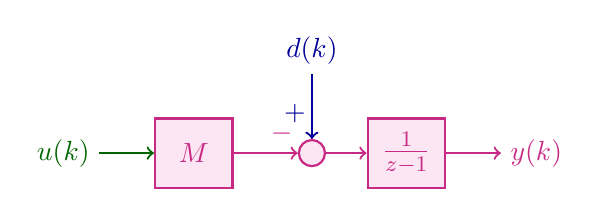
\begin{tikzpicture} [auto, node distance=2cm]

\def\colC{green!40!black};
\def\fillC{green!20!white};

\def\colS{magenta!80!black};
\def\fillS{magenta!10!white};

\def\colE{blue!60!black};
\def\fillE{cyan!20!white};

\node[circle,thick,
      draw=\colS,fill=\fillS]
      (sum) {};

\node[block,thick,
      left of=sum,node distance=1.5cm,
      draw=\colS,fill=\fillS]
      (M) {\textcolor{\colS}{$M$}};

\node[left of=M,\colC,
      anchor=east,node distance=1.2cm]
      (u) {$u(k)$};

\node[above of=sum,\colE,
      anchor=south,node distance=1cm]
      (d) {$d(k)$};

\node[block,thick,
      right of=sum,node distance=1.2cm,
      draw=\colS,fill=\fillS]
      (P) {\textcolor{\colS}{\large{$\frac{1}{z-1}$}}};

\node[right of=P,\colS,
      anchor=west,node distance=1.2cm]
      (y) {$y(k)$};

\draw[->,\colC,thick]
     (u.east) -- (M.west);

\draw[->,\colS,thick]
     (M.east)
      -- node[pos=0.75,above]{$-$}
     (sum.west);

\draw[->,\colE,thick]
     (d.south)
      -- node[pos=0.60,left,xshift=0.5mm]{$+$}
     (sum.north);

\draw[->,\colS,thick]
     (sum.east) -- (P.west);

\draw[->,\colS,thick]
     (P.east) -- (y.west);


\end{tikzpicture}
